\documentclass{article}
\usepackage[ruled,vlined,linesnumbered]{algorithm2e}
\usepackage{algpseudocode}
\usepackage{amsmath}
\usepackage{amsthm}
\usepackage{graphicx}
\usepackage{subfigure}
\usepackage{float}
\usepackage{amsmath }
\usepackage{amsfonts }
\usepackage{pdfpages}
\usepackage{epsfig}
\usepackage{graphicx}
\usepackage{arydshln}
\usepackage{verbatim}
\usepackage{subfigure}
\usepackage{enumerate}
\usepackage{rotating}
\usepackage{threeparttable}
\usepackage{caption}
\usepackage{epsfig}
\usepackage{cite}
\usepackage{times}
\usepackage{geometry}
\usepackage{setspace}
\usepackage[most]{tcolorbox}
\usepackage{tikz}
\usetikzlibrary{trees}
\geometry{a4paper}
\setstretch{1.2}
\usepackage[colorlinks,linkcolor=blue]{hyperref}
\begin{document}
\title{AI3613 Database System Concepts Homework 3}
\author{Kailing Wang 521030910356}
\date{May 9.2024}
\maketitle

\section*{Problem 1}

\begin{enumerate}[1.]
	\item
	      \begin{enumerate}[(a)]
		      \item In this case, all 300 pages are needed to read from disk. Every page can contain touples where there are students with gpa>3.7.
		      \item 100 pages are needed to read from disk. We only have to go over the gpa row and count. We do not need to know the name and id.
	      \end{enumerate}

	\item
	      \begin{enumerate}[(a)]
		      \item In this case, we'd stop on finding a touple with id=123. The most lucky case is that the first page contains the touple. The worst case is that the last page contains the touple. The pages we need to read from disk range from 1 to 300.
		      \item Similarly, we first scan the id row to find the offset for id=123. The pages we need to read from disk range from 1 to 100. Then we read two more pages to get the name and gpa. The total pages we need to read from disk range from 3 to 102.
	      \end{enumerate}
\end{enumerate}

\section*{Problem 2}
\begin{enumerate}[(1)]
	\item Put 8 into the tree
	      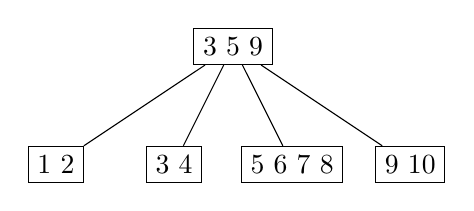
\begin{tikzpicture}[scale=1, every node/.style={rectangle, draw}]
		      \node {3 5 9}
		      child {node {1 2}}
		      child {node {3 4}}
		      child {node {5 6 7 8}}
		      child {node {9 10}};
	      \end{tikzpicture}

	      Split the leaf node
	      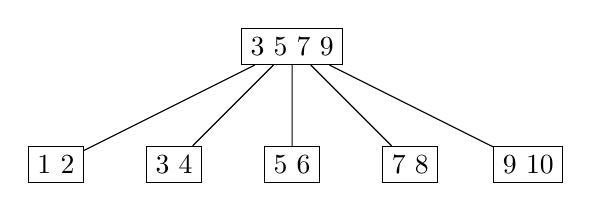
\begin{tikzpicture}[scale=1, every node/.style={rectangle, draw}]
		      \node {3 5 7 9}
		      child {node {1 2}}
		      child {node {3 4}}
		      child {node {5 6}}
		      child {node {7 8}}
		      child {node {9 10}};
	      \end{tikzpicture}

	      Split the root node
	      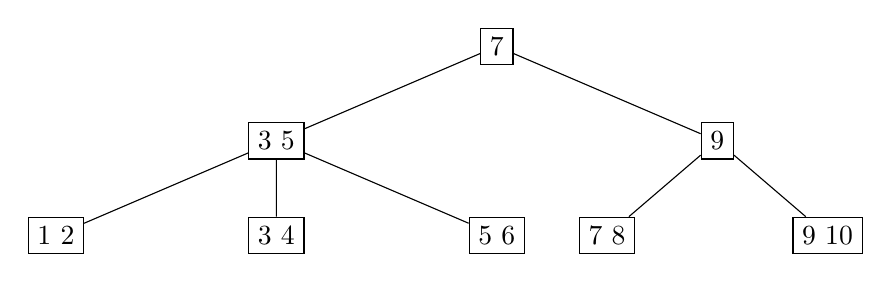
\begin{tikzpicture}[scale=0.8,
			      level 1/.style={sibling distance=70mm, level distance=15mm},
			      level 2/.style={sibling distance=35mm, level distance=15mm},
			      every node/.style={rectangle, draw}]
		      \node {7}
		      child {node {3 5}
				      child {node {1 2}}
				      child {node {3 4}}
				      child {node {5 6}}
			      }
		      child {node {9}
				      child {node {7 8}}
				      child {node {9 10}}
			      };
	      \end{tikzpicture}
	\item Delete 7 from the tree
	      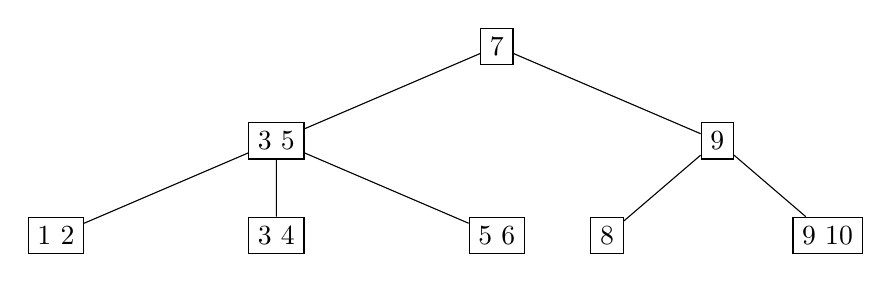
\begin{tikzpicture}[scale=0.8,
			      level 1/.style={sibling distance=70mm, level distance=15mm},
			      level 2/.style={sibling distance=35mm, level distance=15mm},
			      every node/.style={rectangle, draw}]
		      \node {7}
		      child {node {3 5}
				      child {node {1 2}}
				      child {node {3 4}}
				      child {node {5 6}}
			      }
		      child {node {9}
				      child {node {8}}
				      child {node {9 10}}
			      };
	      \end{tikzpicture}

	      According to the rule, merge with the left sibling
	      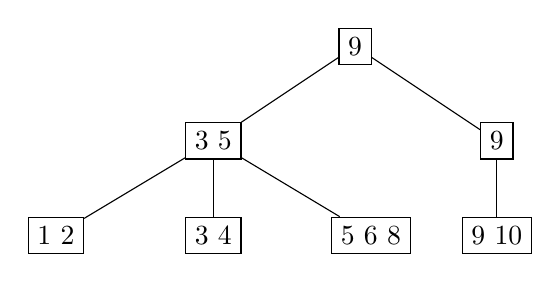
\begin{tikzpicture}[scale=0.8,
			      level 1/.style={sibling distance=45mm, level distance=15mm},
			      level 2/.style={sibling distance=25mm, level distance=15mm},
			      every node/.style={rectangle, draw}]
		      \node {9}
		      child {node {3 5}
				      child {node {1 2}}
				      child {node {3 4}}
				      child {node {5 6 8}}
			      }
		      child {node {9}
				      child {node {9 10}}
			      };
	      \end{tikzpicture}

	      Merge the internal node
	      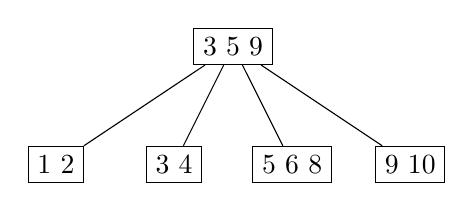
\begin{tikzpicture}[scale=1, every node/.style={rectangle, draw}]
		      \node {3 5 9}
		      child {node {1 2}}
		      child {node {3 4}}
		      child {node {5 6 8}}
		      child {node {9 10}};
	      \end{tikzpicture}
	\item 1.read root node, 1 page

	      2. find the leaf node that contains the key 2, 1 page

	      3. use the tail pointer to fing the (3, 4) node, 1 page

	      4. again to the 5, 6, 8 node, 1 page

	      In total, 4 pages are needed to read from disk.
\end{enumerate}

\section*{Problem 3}
\begin{tcolorbox}[colback=gray!10, breakable]
	How long does it take you to finish the assignment? Give a score (1,2,3,4,5) to the difficulty of each problem. List all your collaborators if you have any.
\end{tcolorbox}

I'm extremely busy this recently so I only assign 1 hour to this homework, and I think it might actually took less. Rate 2, 2.
\end{document}